\section{H-Brücke}\label{Appendix:H_Bruecke}

\subsection{Referenzschema}\label{Appendix:H_Bruecke_Referenzschema}

\begin{figure}[h!]
	\centering
	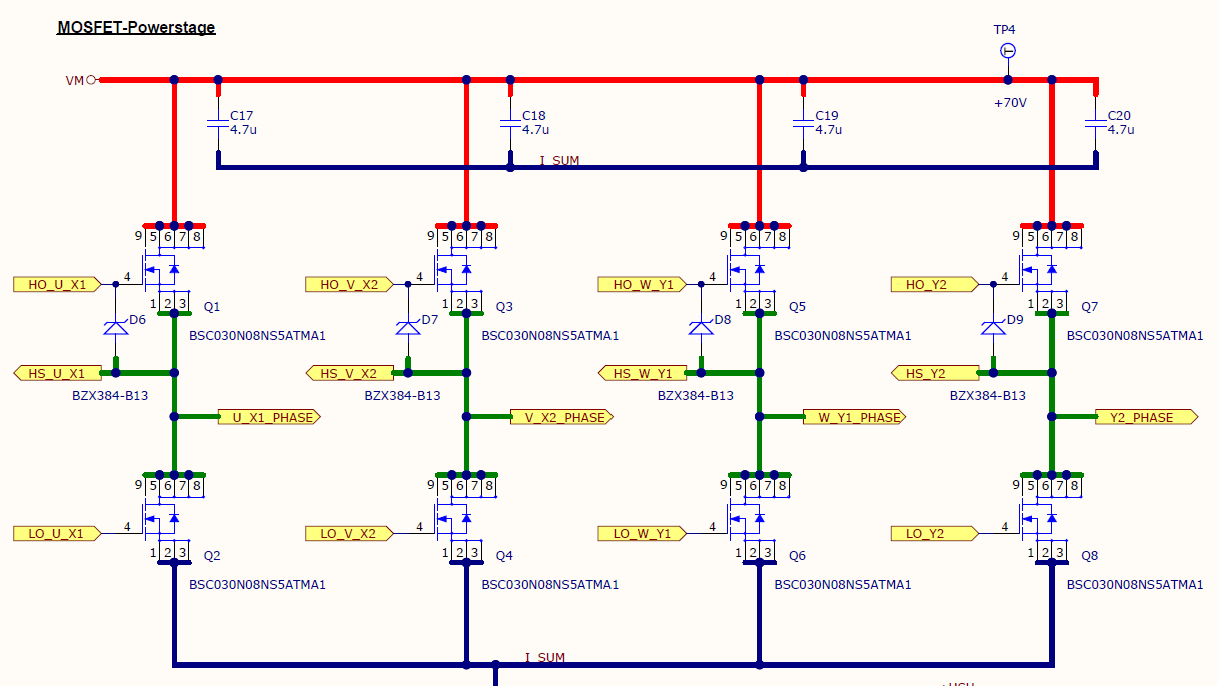
\includegraphics[width=0.9\textwidth]{graphics/Referenzschema_10A70V}
	\caption{H-Brücke.}
	\label{fig:Schema_H_Bruecke_und_BLDC_Ref}
\end{figure}

%\todo{cite: Datenblatt UPS 10A70V Schema}

\subsection{Inbetriebnahme}

\subsubsection{Inbetriebnahme Setup}\label{Appendix:H_Bruecke_Setup}

\begin{figure}[h!]
	\centering
	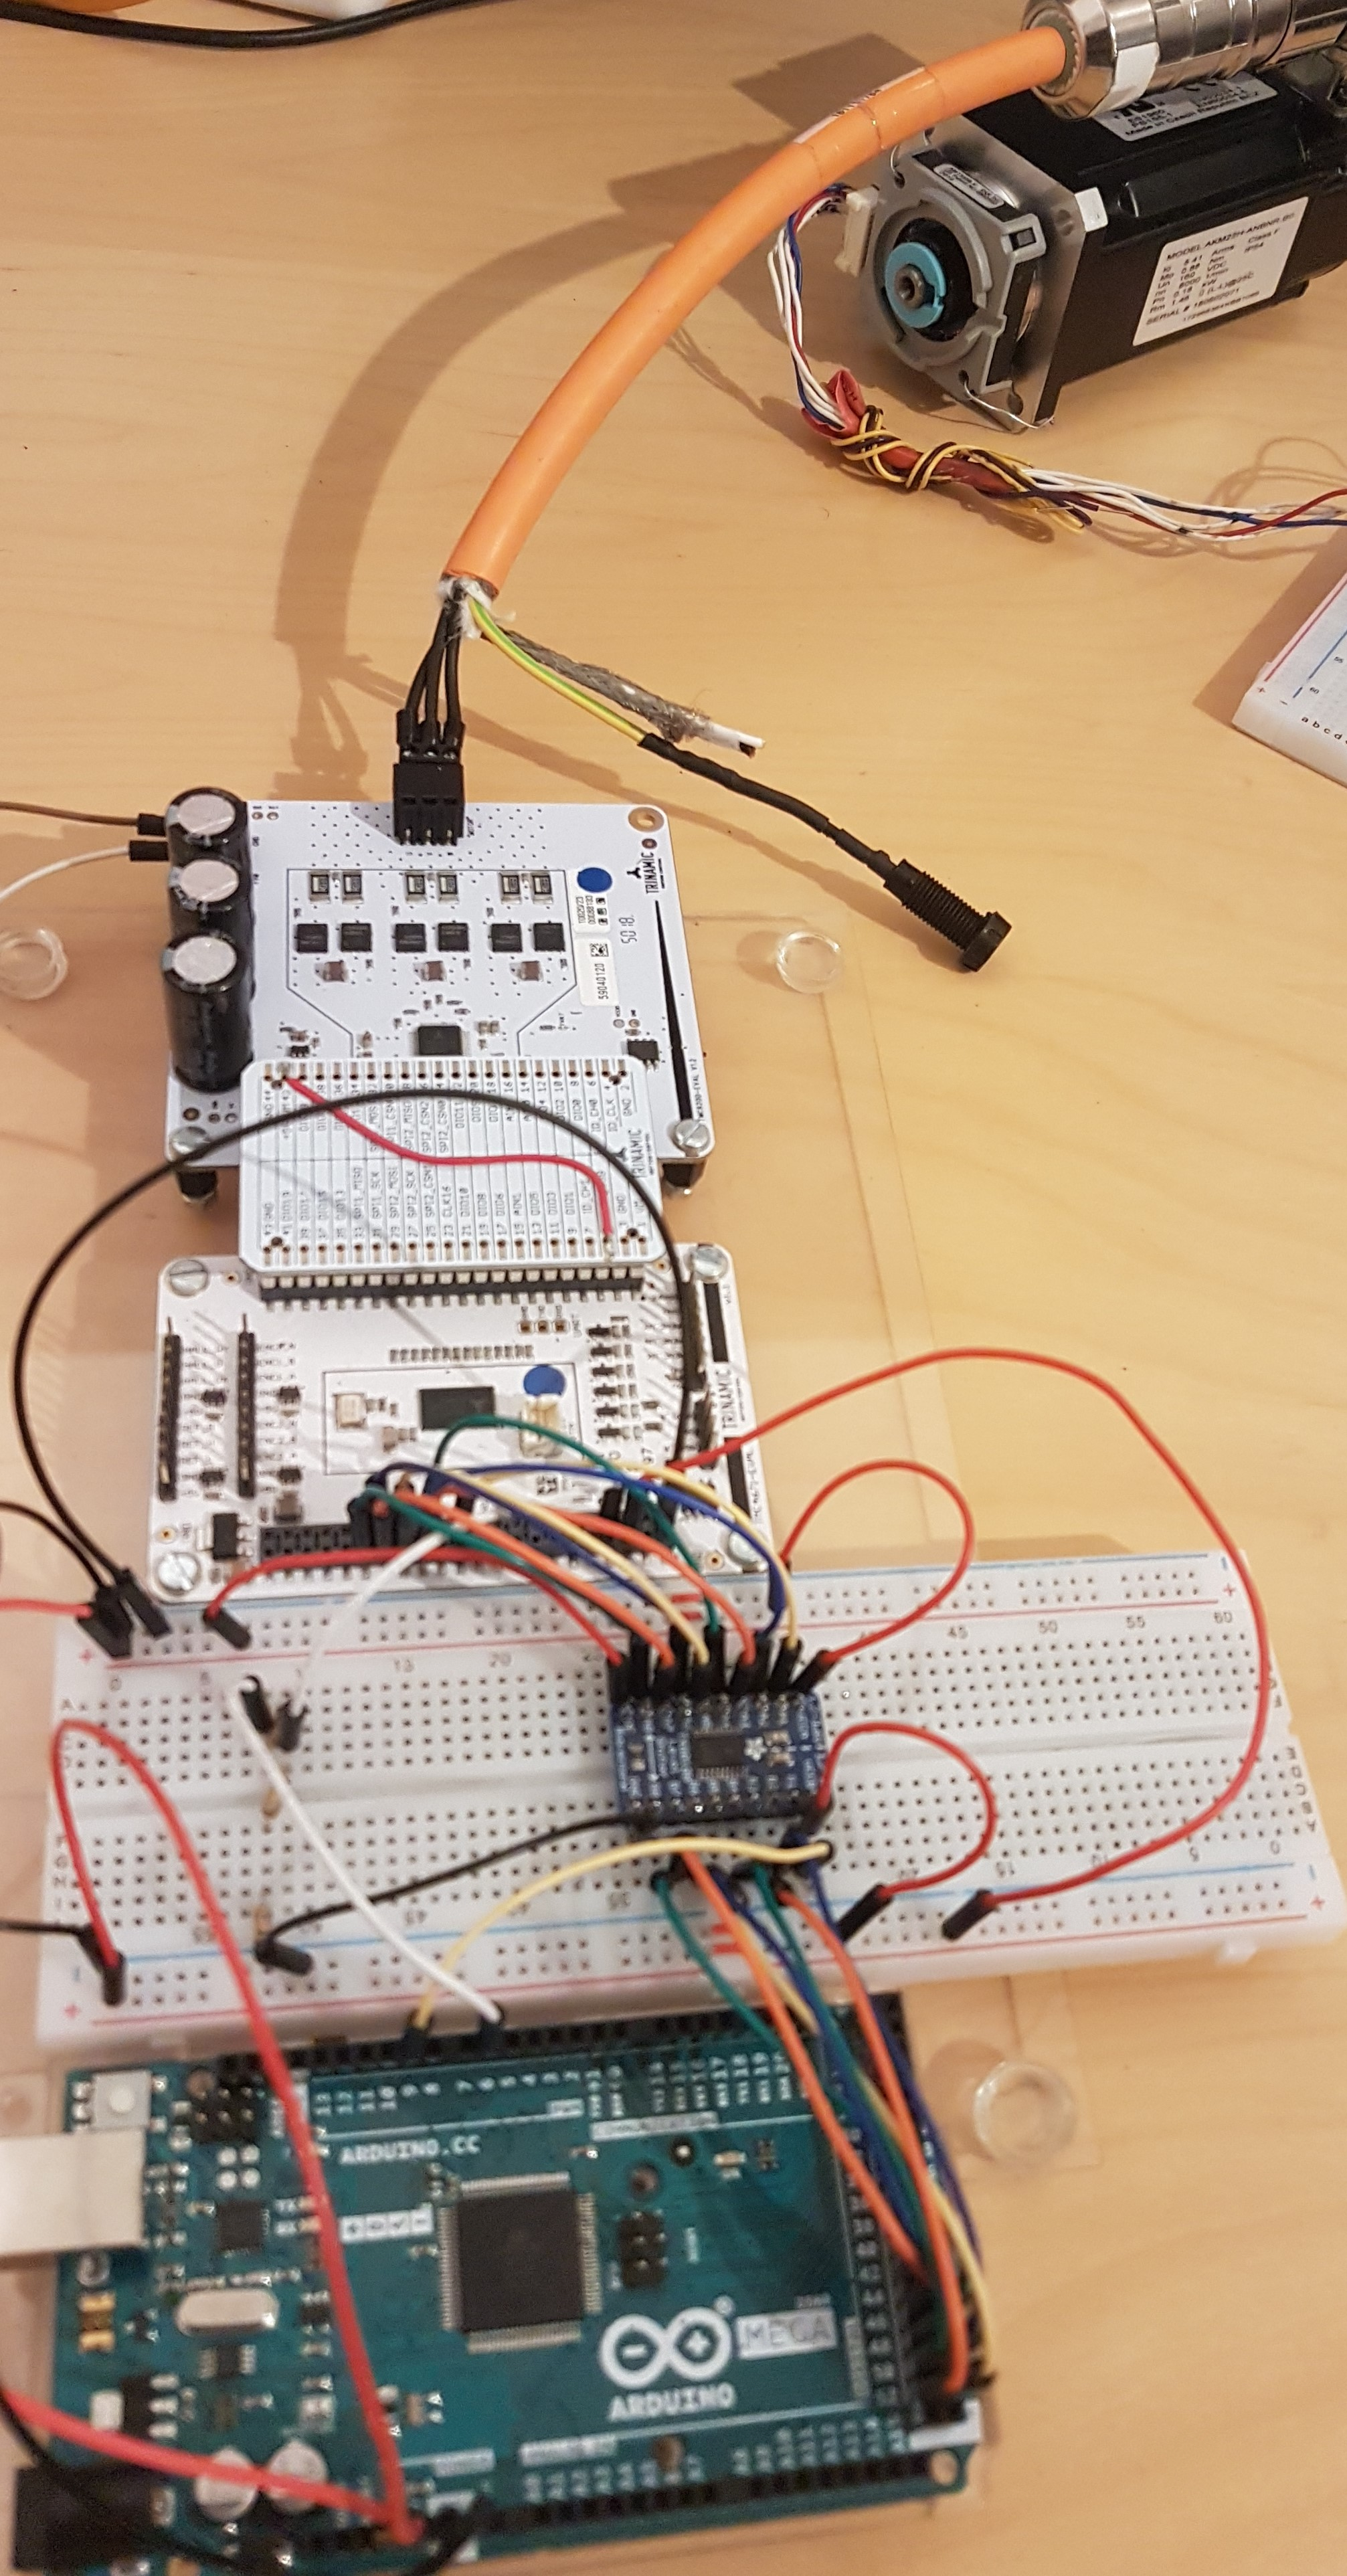
\includegraphics[angle =270, width=0.9\textwidth]{graphics/3_normal}
	\caption{Setup Inbetriebnahme H-Brücke und Motor.}
	\label{fig:3_normal}
\end{figure}

\newpage

\subsubsection{Inbetriebnahme Schaltsignale}\label{Appendix:H_Bruecke_Schaltsignale}

\begin{figure}[h!]
	\centering
	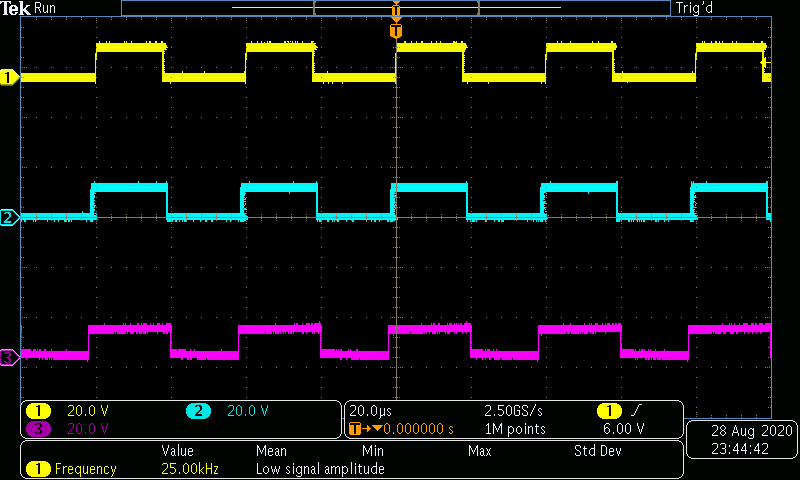
\includegraphics[width=\textwidth]{graphics/OpenLoop_TestDrive2}
	\caption{Schaltsignale während dem Openloop Testdrive. Gelb = U, Blau = V, Magenta = W}
	\label{fig:OpenLoop_TestDrive2}
\end{figure}